\section{محاسبه برش پانچ در \lr{FreeCAD}}

\subsection{بارگذاری ورک بنچ \lr{Civil}\label{sec:loadingcivil}}
بعد از باز کردن نرم افزار 
\lr{FreeCAD}
، مطابق شکل
\ref{fig:civil-workbench}
با کلیک روی منوی کرکره ای ورک بنچ ها، از لیست موجود 
\lr{Civil}
را انتخاب کنید. با این کار منو و آیکون های نرم افزار برش پانچ ظاهر میشوند. برای اینکه هر دفعه پس از بازکردن نرم افزار نیاز به این کار نداشته باشید به قسمت
\ref{faq}
 مراجعه کنید.

\begin{figure}[H]
    \centering
    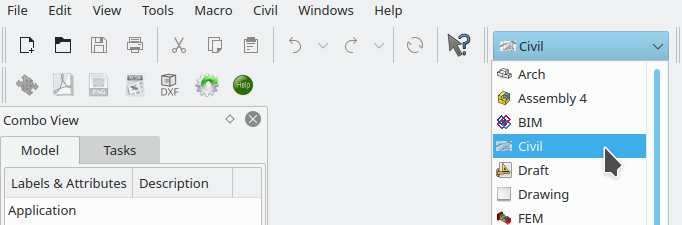
\includegraphics[width=\linewidth]{figures/civil}
    \caption{بارگذاری ورک بنچ \lr{Civil}}
    \label{fig:civil-workbench}
\end{figure}
\subsection{بازکردن فایل اکسل}
برای فراخوانی فایل اکسلی که در بخش 
\ref{sec:prepare-safe}
ساختیم، کافیست که آنرا مثل یک فایل اکسل در نرم افزار باز کنید. یعنی از منوی
$File \rightarrow Open$
این کار را انجام دهید. در این مرحله حتی نیاز به فراخوانی ورک بنچ 
\lr{Civil}
نمی باشد. بعد از چند لحظه فنداسیون داخل نرم افزار بارگذاری شده و محاسبات پانچ برای تمامی ستونها صورت میگیرد.

\subsection{ذخیره پروژه}
در ورژن جدید میتوانید به سادگی مثل سایر نرم افزارها پروژه را ذخیره و باز کنید. بعد از بازکردن پروژه های ذخیره شده میتوانید ویرایش های لازم را انجام دهید. این قابلیت در 
ورژن های قبلی نرم افزار موجود نبود.